% !TEX encoding = UTF-8 Unicode
% -*- coding: UTF-8; -*-
% vim: set fenc=utf-8

% REVIEW: {referencial, embasamento} teórico
\chapter{Referencial Teórico}%
\label{chap:referencial-teorico}

\perrotta{Capítulo 02 --- Referencial Teórico}

Nessa seção serão abordados alguns conceitos e a terminologia que será utilizada ao longo desse trabalho.

\section{Conceitos básicos}

\section{Especificações}%
\label{sec:especificacoes}

\subsection{Dataflow}

Uma especificação de fluxo de dados \( D_F \) é definida como \[ D_F = (T, S, \Phi) \] onde:
\begin{itemize}
    \item \( T = \{t_1, t_2, \ldots, t_{\alpha}\} \) \vdots{}
    \( \{t_i \mid i \in \{{1, 2, \ldots, \alpha}\} \} \)
    é transformação
    \item \( S = \{s_1, s_2, \ldots, t_{\beta}\} \) \vdots{}
    \( \{s_i \mid i \in \{{1, 2, \ldots, \beta}\} \} \)
    é conjunto de dados
    \item \( \Phi = \{\phi_1, \phi_2, \ldots, \phi_{\gamma}\} \) \vdots{}
    \( \{\phi_i \mid i \in \{{1, 2, \ldots, \gamma}\} \} \){}
    é dependência de dados
\end{itemize}

\missingfigure{Exemplo de -> o ->, i.e., transformação com dataset de entrada e de saída}

\perrotta{Acho que falta definir o que é uma transformação.}

\subsection{Dependência de dados}

Uma especificação de dependência de dados \( \phi \) é definida como \[ \phi = (s, t_{\textrm{previous}}, t_{\textrm{next}}) \] onde:
\begin{itemize}
    \item \( s \) é um conjunto de dados
    \item \( t_{\textup{previous}} \) é a transformação que {\bf produz} dados para o conjunto de dados \( s \)
    \item \( t_{\textup{next}} \) é a transformação que {\bf consome} dados do conjunto de dados \( s \)
\end{itemize}

\subsection{Conjunto de dados}

A especificação de um conjunto de dados \( s \) é dada por \[ s = (A, C) \] onde:
\begin{itemize}
    \item \( A = \{a_1, a_2, \ldots, a_{\delta} \} \; \vdots{} \; \{ a_i \mid i \in \{1, 2, \ldots, \delta \} \} \) é atributo
    \item \( C = \{c_1, c_2, \ldots, c_{\zeta} \} \; \vdots{} \; \{ c_i \mid i \in \{1, 2, \ldots, \zeta \} \} \) é coleção de dados
\end{itemize}

\subsection{Atributo}

Um atributo é especificado da seguinte forma: \[ a = (\textrm{nome},\textrm{tipo}) \therefore \textrm{tipo} = \{\textup{inteiro}, \textup{ponto flutuante}, \textup{texto}, \textup{arquivo}\} \]

\subsection{Coleção de dados}

Uma coleção de dados é definida como \[ c = \{ i_1, i_2, \ldots, i_{\eta} \} \; \vdots \; \{ i_j \mid j \in \{ 1, 2, \ldots, \eta \} \} \] é item de dados

\subsection{Item de dados}

A especificação de um item de dados é dada por \[ i = (s, T^{\ast}_{\textrm{previous}}, T^{\ast}_{\textrm{next}}, e) \] onde:

\begin{itemize}
    \item \( s \) é um conjunto de dados
    \item \( T^{\ast}_{\textrm{previous}} \) é o conjunto com todas as instâncias de todas as transformações que são responsáveis por gerar \( i \)
    \item \( T^{\ast}_{\textrm{next}} \) é o conjunto com todas as instâncias de todas as transformações que consomem \( i \)
    \item \( e \) é um elemento de dados
\end{itemize}

\subsection{Elemento de dados}

Um elemento de dados é definido como

\[ e = \{ v_1, v_2, \ldots, v_{\theta} \} \therefore \#(s.A) = \#(e) \]
\[ v_{\theta} \; \textrm{é o valor do atributo} \; a_{\theta} \; \textrm{de um item de dados do conjunto de dados} \; s \]

onde \( \#(S) \) representa a cardinalidade do conjunto \( S \), i.e.\ a quantidade de elementos presentes no mesmo.

\section{Um exemplo}

Para ilustrar as definições e especificações da \autoref{sec:especificacoes}, vamos utilizar uma pequena amostra do conjunto de dados de sedimentação. Na \autoref{fig:example-dataflow-specification} \perrotta{expandir comentário sobre a figura}

\begin{figure}[ht]
    \centering
    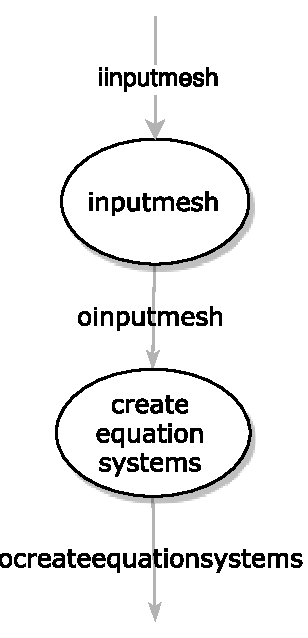
\includegraphics[width=0.35\textwidth]{img/example-dataflow-specification}
    \caption[Exemplo de especificação de fluxo de dados]{Exemplo de especificação de fluxo de dados, com duas transformações e três conjuntos de dados.}%
    \label{fig:example-dataflow-specification}
\end{figure}

\missingfigure{Incluir um exemplo, com figuras, de um pequeno dataflow.}

\[
\begin{aligned}
D_F = && (T, S, \Phi) \\
T = && \{ \textrm{inputmesh} \} \\
S = && \{ \textrm{iinputmesh}, \textrm{oinputmesh} \} \\
\Phi = && \{ (\textrm{nil}, \textrm{iinputmesh}, \textrm{inputmesh}),
(\textrm{inputmesh}, \textrm{oinputmesh}, \textrm{nil})
\} \\
\end{aligned}
\]

\perrotta{Capítulo 02 --- misc}

%%%%%%%%%%%%%%%%%%%%%%
% Simulações computacionais
% (OK) Fluxo de dados = dataflow - definições {d,n}o outro google docs
% Proveniência de dados
% Gerência do fluxo de dados
% Mecanismos para processamento de consultas
